This test problem is a 2-D dam break problem for the shallow
water equations. In this test problem, a walled, H-shaped region
(from $x=0$ to $x=6$ and from $y=0$ to $y=6$) is initially dammed at $x=4$,
from $y=2$ to $y=4$,
until at $t=0$, the dam breaks. Water flows into what will be
referred to as the ``reservoir'' region, to the right of $x=4$.
Figure \ref{fig:dam_break_2d_initial} illustrates the initial height profile
for this test problem and the H-shaped problem domain. The initial velocity
is zero everywhere.
The problem parameters are summarized in Table \ref{tab:dam_break_2d}.

%-------------------------------------------------------------------------------
\begin{figure}[htb]
   \centering
   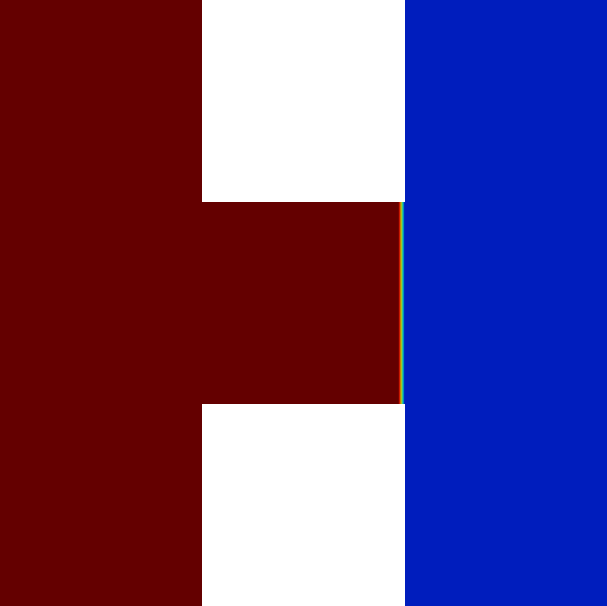
\includegraphics[width=\textwidth]
     {\contentdir/results/shallowwater/dam_break_2d/images/initial.png}
   \caption{Initial Height Profile for the 2-D Dam Break Test Problem}
   \label{fig:dam_break_2d_initial}
\end{figure}
%-------------------------------------------------------------------------------

%-------------------------------------------------------------------------------
\begin{table}[htb]\caption{2-D Dam Break Test Problem Summary}
\label{tab:dam_break_2d}
\centering
\begin{tabular}{l l}\toprule
\emph{Parameter} & \emph{Value}\\\midrule
Domain & $\mathcal{D} = ((0,2)\times(0,6))\cup((2,4)\times(2,4))\cup((4,6)\times(0,6))$\\
Initial Conditions & $\height_0(\x)=\left\{\begin{array}{c l}
    0.05 & x < 4\\
    0.01 & x >= 4
  \end{array}\right.$\\
                   & $\velocity_0(\x) = \mathbf{0}$\\
Boundary Conditions & $\nabla\height(\x,t)=0
  \eqc \quad \x\in\partial\mathcal{D}\eqc \quad t>0$,\\
                    & $\velocity\xt\cdot\normalvector = 0
  \eqc \quad \x\in\partial\mathcal{D}\eqc \quad t>0$,\\
Bathymetry & $\bathymetry(\x)=0$\\
Gravity    & $\gravity=0.05$\\
\bottomrule\end{tabular}
\end{table}
%-------------------------------------------------------------------------------

This simulation was run using the low-order invariant domain method and
the entropy viscosity method to $t=50$, using the SSPRK33 time discretization.
The run parameters for this test problem are summarized in Table
\ref{tab:dam_break_2d_run}.

%-------------------------------------------------------------------------------
\begin{table}[htb]\caption{2-D Dam Break Test Problem Run Parameters}
\label{tab:dam_break_2d_run}
\centering
\begin{tabular}{l l}\toprule
\emph{Parameter} & \emph{Value}\\\midrule
Number of Cells & $N_{cell} = 7168$\\
End Time        & $t=50$\\
CFL Number      & $\nu=0.05$\\
Time Integrator & SSPRK33\\\midrule
Entropy Residual Coefficient & $\entropyresidualcoef=1$\\
Entropy Jump Coefficient & $\entropyjumpcoef=1$\\
\bottomrule\end{tabular}
\end{table}
%-------------------------------------------------------------------------------

Figure \ref{fig:dam_break_2d_height} compares the height color maps for
the low-order and high-order schemes, and Figure \ref{fig:dam_break_2d_surface} 
shows the height surfaces, colored by the magnitude of the momentum.
The entropy viscosity solution shows a much less diffusive solution - note
for example, the ``negative'' wave front to the left of $x=2$, the sharpness
of the wave front in the reservoir region to the right of $x=4$, and the height
of the reflected wave hitting the right boundary of the reservoir region.
However, note the presence of some spurious oscillations at the interior corners
along $x=2$ in the surface plot of the entropy viscosity solution. These
interior corners, and especially the interior corners along $x=4$, where
the initial discontinuity lies, are challenging regions and tend to give rise to
severe oscillations if the time step size is too large. In these simulations,
a CFL as small as $\nu=0.1$ was shown to give an unstable solution, so a
CFL of $\nu=0.05$ was used. Figures \ref{fig:dam_break_2d_visc} shows
the low-order and entropy viscosity profiles, both on logscales (but separately
scaled). From the entropy viscosity profile, one can see that the interior
corner cells have the highest entropy viscosities, followed by the wave
front in the reservoir region and its reflected wave.

%-------------------------------------------------------------------------------
\begin{figure}[htb]
   \centering
   \begin{subfigure}{0.45\textwidth}
     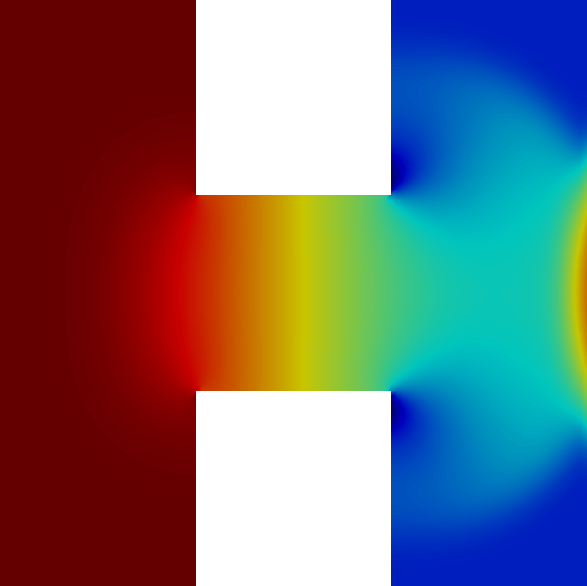
\includegraphics[width=\textwidth]
       {\contentdir/results/shallowwater/dam_break_2d/images/height_Low.png}
     \caption{Low-order scheme}
   \end{subfigure}
   \begin{subfigure}{0.45\textwidth}
     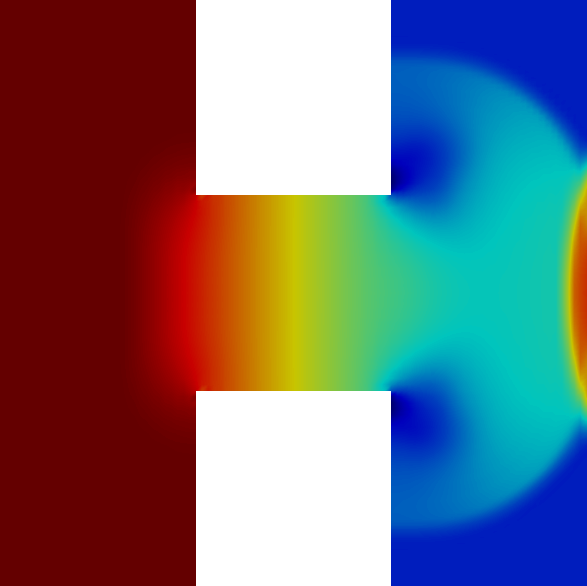
\includegraphics[width=\textwidth]
       {\contentdir/results/shallowwater/dam_break_2d/images/height_EV.png}
     \caption{High-order scheme}
   \end{subfigure}
   \caption{Comparison of Height Solutions for the 2-D Dam Break Test Problem}
   \label{fig:dam_break_2d_height}
\end{figure}
%-------------------------------------------------------------------------------
\begin{figure}[htb]
   \centering
   \begin{subfigure}{0.45\textwidth}
     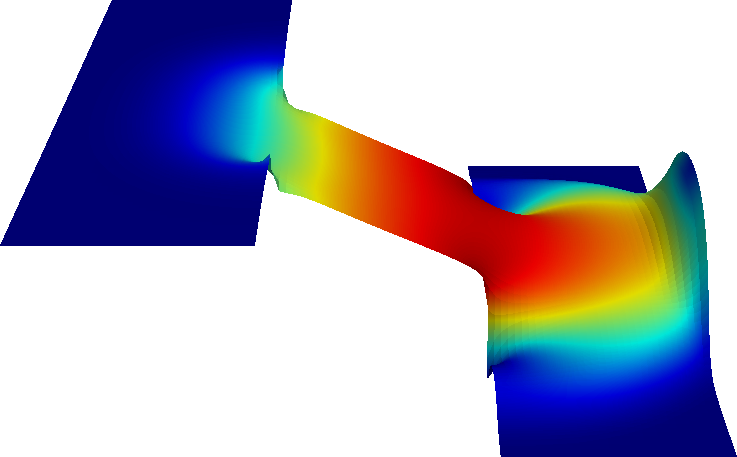
\includegraphics[width=\textwidth]
       {\contentdir/results/shallowwater/dam_break_2d/images/height_Low_surface.png}
     \caption{Low-order scheme}
   \end{subfigure}
   \begin{subfigure}{0.45\textwidth}
     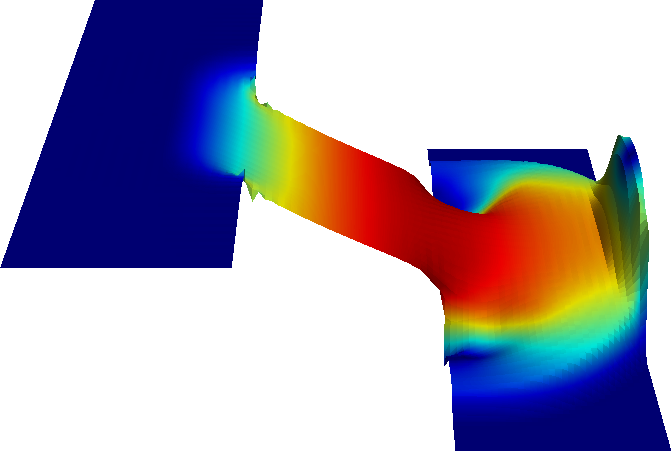
\includegraphics[width=\textwidth]
       {\contentdir/results/shallowwater/dam_break_2d/images/height_EV_surface.png}
     \caption{High-order scheme}
   \end{subfigure}
   \caption{Comparison of Solution Surfaces for the 2-D Dam Break Test Problem}
   \label{fig:dam_break_2d_surface}
\end{figure}
%-------------------------------------------------------------------------------
\begin{figure}[htb]
   \centering
   \begin{subfigure}{0.45\textwidth}
     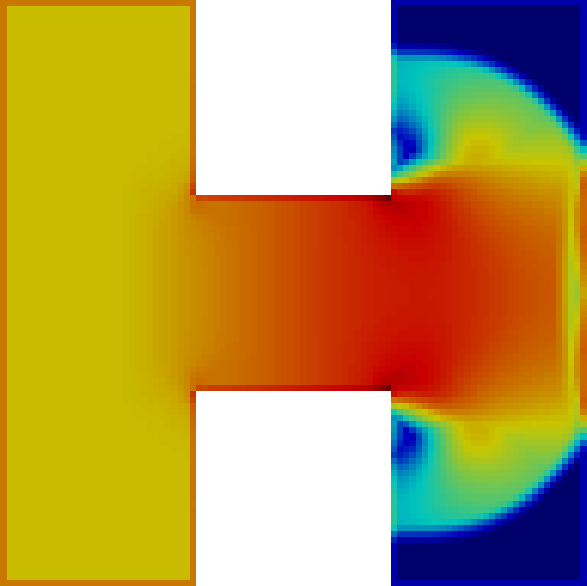
\includegraphics[width=\textwidth]
       {\contentdir/results/shallowwater/dam_break_2d/images/low_order_viscosity_logscale.png}
     \caption{Low-order Viscosity}
   \end{subfigure}
   \begin{subfigure}{0.45\textwidth}
     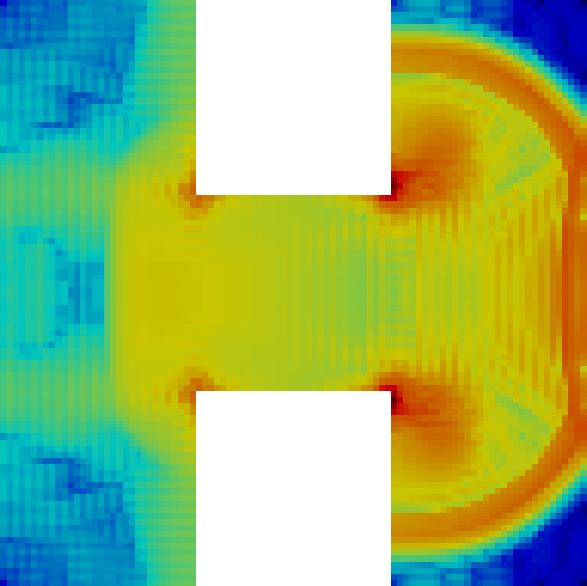
\includegraphics[width=\textwidth]
       {\contentdir/results/shallowwater/dam_break_2d/images/entropy_viscosity_logscale.png}
     \caption{Entropy Viscosity}
   \end{subfigure}
   \caption{Comparison of Viscosity Profiles for the 2-D Dam Break Test Problem}
   \label{fig:dam_break_2d_visc}
\end{figure}
%-------------------------------------------------------------------------------

\clearpage
